\section{Strumenti: ricerca}
Giallozafferano è un sito web contenente moltissima informazione, divisa in tantissime pagine raggruppate in sezioni; la ricerca è dunque uno strumento fondamentale e necessario anche per risolvere il problema della \textbf{long tail}, cioè il fenomeno per cui solo poche pagine ottengono circa l'80\% dell'attenzione. Si stima inoltre che la ricerca venga utilizzata circa nel 60\% dei casi di deep linking, dato che gli utenti sono abituati ai motori di ricerca.
Il sito in esame è inoltre frequentemente aggiornato, è dunque cruciale l'utilizzo di un buon motore di ricerca, dato che spesso i menù da soli non riescono a seguire gli aggiornamenti.
\\~\textbf{Premessa}: quando si è analizzata la pagina della ricetta, si è fatto notare la presenza di una barra di ricerca alla fine di tale pagina; dato che essa è presente solo in quella tipologia di pagina e come detto sarà vista da pochissimi utenti, si è deciso di non considerarla.
\\~Come si può vedere in una qualsiasi delle schermate presenti nelle sezioni precedenti, la ricerca è posizionata in alto a destra, posizione perfetta. Essa è composta da un box testuale che supporta un numero massimo di 26 caratteri prima che uno di essi venga nascosto: non sono molti, ma potrebbero essere sufficienti a soddisfare una percentuale abbastanza elevata di utenti (con 30 caratteri è soddisfatto circa l'80\% degli utenti); la grandezza del search box è fondamentale, poiché per ogni carattere nascosto aumenta proporzionalmente lo stress e l'utente medio tende inconsciamente a rimanere entro il limite imposto, scrivendo query meno specifiche che portano a risultati più scarsi. Visto lo spazio a disposizione, sarebbe stato più saggio utilizzare un box dinamico che aumenta in grandezza non appena l'utente vi clicca sopra.
\\~Altro punto fondamentale è il pulsante di ricerca: giallozafferano opta per l'utilizzo del simbolo della lente di ingrandimento, cosa abbastanza popolare nel web ma più adatta ad un sito mobile: ancora una volta, vista la quantità di spazio a disposizione, sarebbe stato meglio utilizzare un pulsante con scritto "\textit{cerca}" o "\textit{search}".

\subsection{Pagina dei risultati}

\begin{figure}[h!]
	\centering
	\begin{subfigure}[b]{0.4\textwidth}
		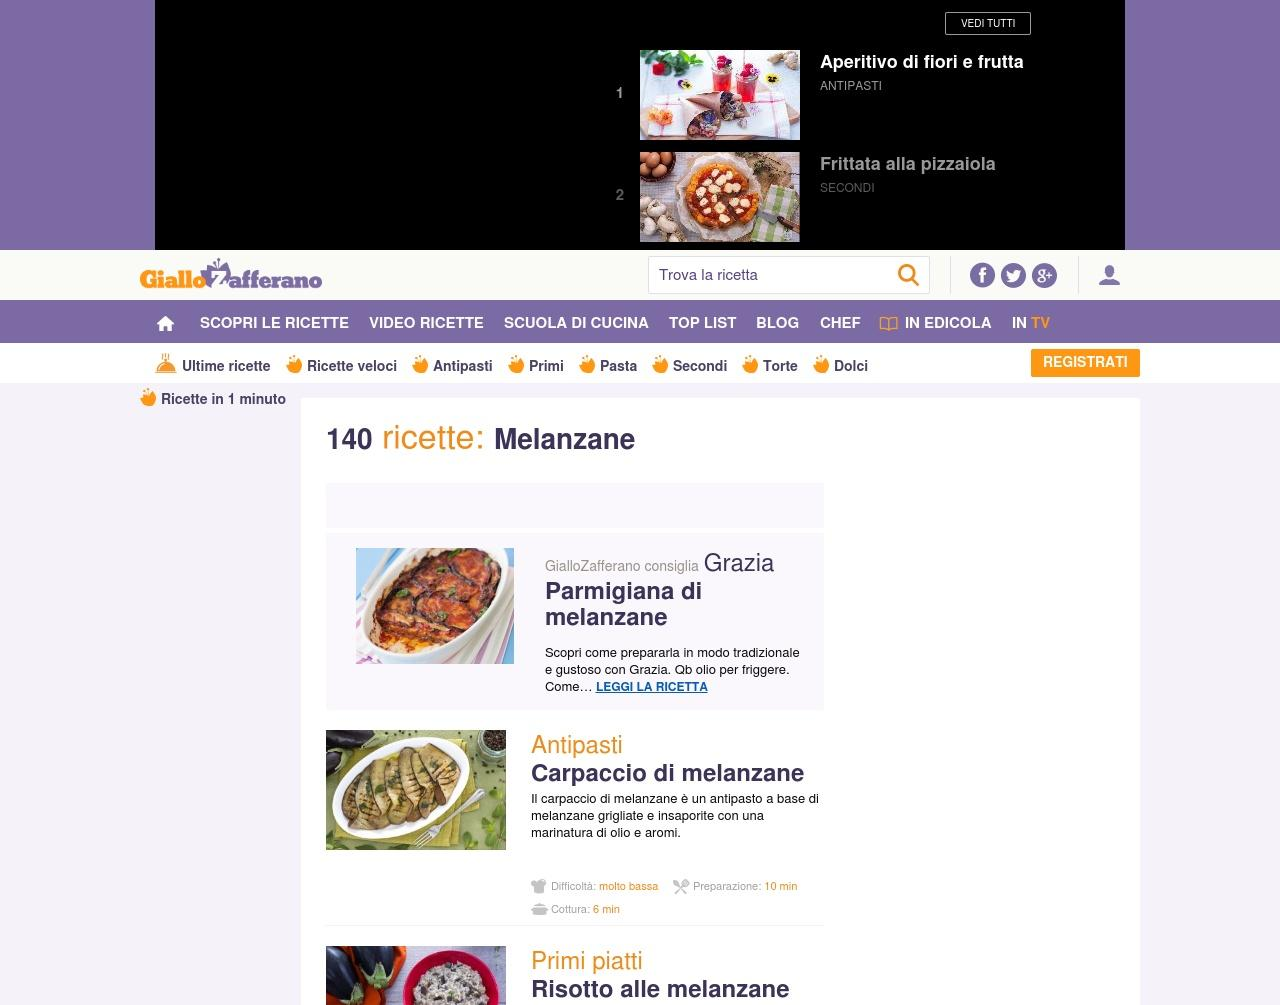
\includegraphics[scale=0.1]{images/risultati/risultati-0.jpeg}
		\subcaption{}
	\end{subfigure}
	\begin{subfigure}[b]{0.4\textwidth}
		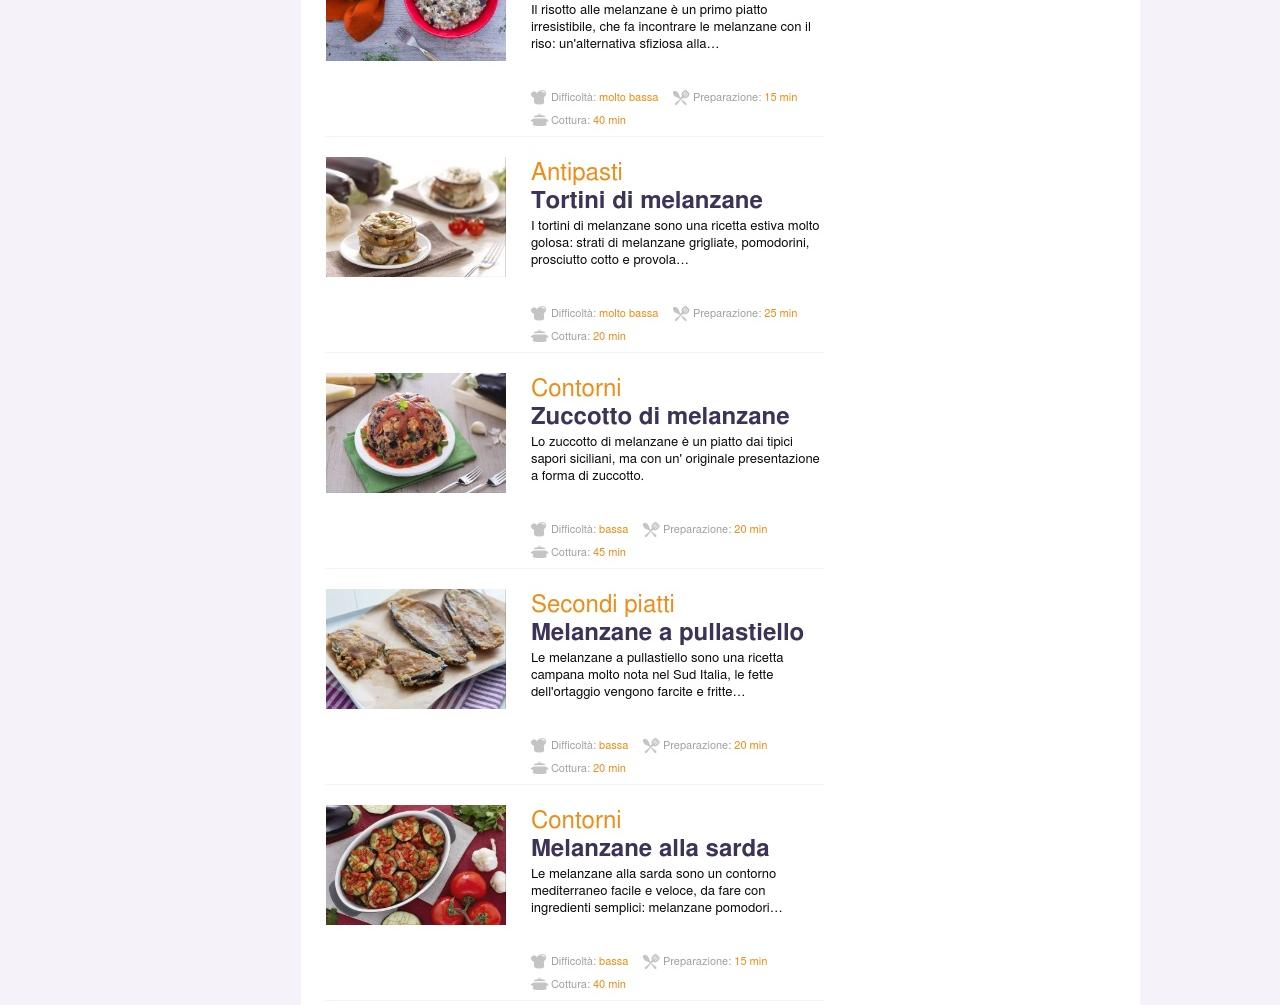
\includegraphics[scale=0.1]{images/risultati/risultati-1.jpeg}
		\subcaption{}
	\end{subfigure}
	\begin{subfigure}[b]{0.4\textwidth}
		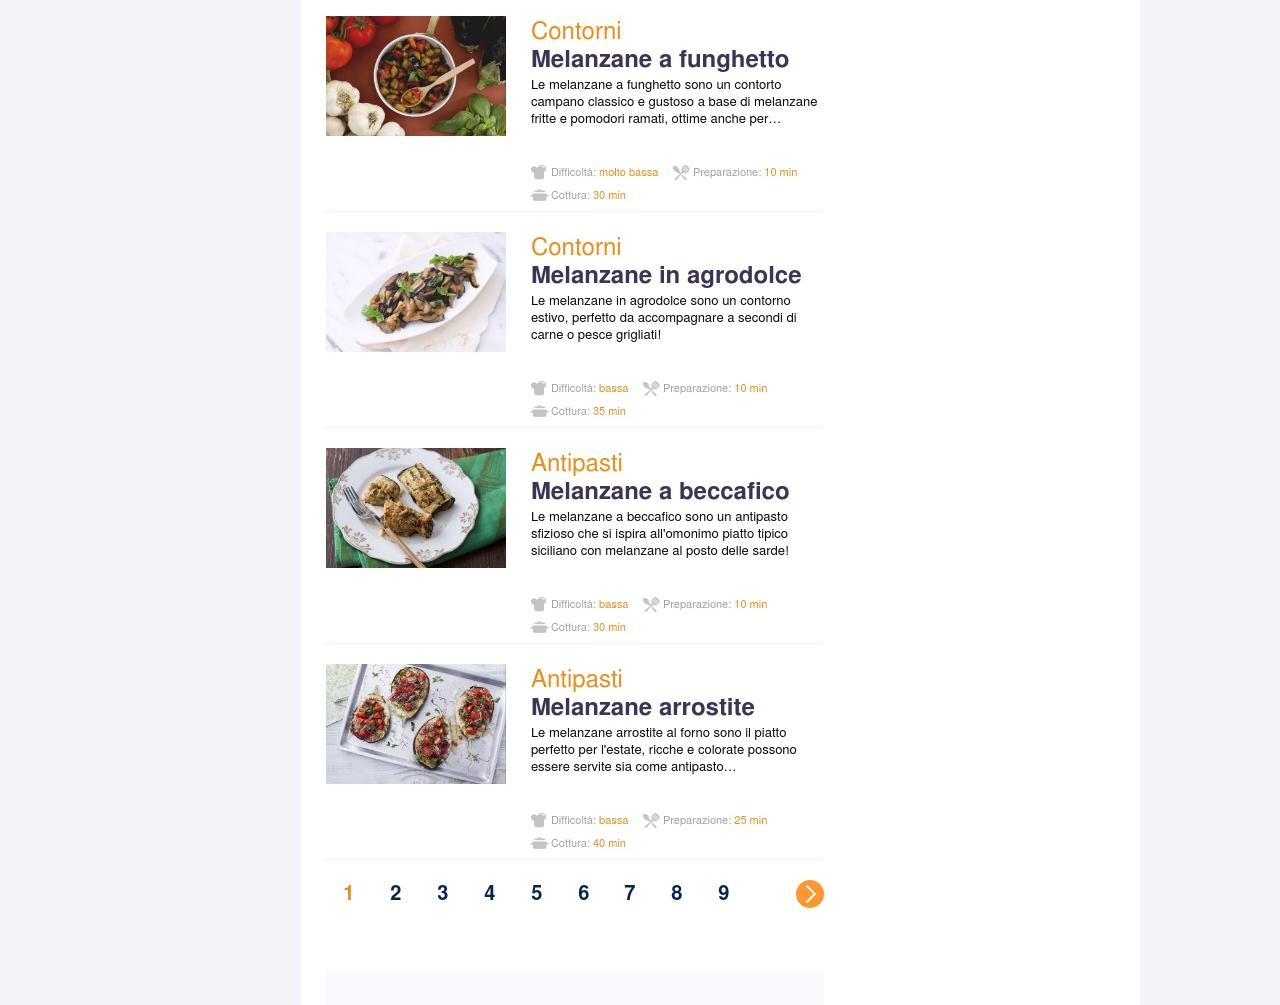
\includegraphics[scale=0.1]{images/risultati/risultati-2.jpeg}
		\subcaption{}
	\end{subfigure}
	\caption{Pagina dei risultati della query "melanzane" (risultati-0,1,2.png) -\newline https://www.giallozafferano.it/ricerca-ricette/melanzane/}
	\label{fig:risultati}
\end{figure}

Le immagini precedenti mostrano la pagina a cui si viene rimandati nel momento in cui si effettua una ricerca: notiamo che come prima cosa viene specificato il numero di risultati trovati, con la sintassi "\textit{Numero ricette: query}"; ciò è sicuramente un'informazione importante, soprattutto nel caso di 0 risultati, poiché chiarisci all'utente se la ricerca è andata a buon fine oppure no.
I risultati vengono presentati in lista: ciò permette di specificare più informazioni riguardo ogni singolo risultato, tuttavia fa un cattivo uso dello spazio, allungandosi in verticale e dividendo i risultati in molte pagine diverse; l'utilizzo di una griglia, in questo caso, sarebbe stata la scelta migliore perché avrebbe compattato l'informazione, permettendo una visualizzazione di più risultati in meno spazio. 
Un'altra cosa che manca è l'aggiunta della ricerca vincolata: dato che le ricette possono essere divise (e sono divise all'interno del sito) in categorie diverse, viene naturale pensare all'introduzione di filtri di ricerca, che aiuterebbero l'utente a trovare esattamente ciò che gli interessa, soprattutto in caso di molti risultati.
Manca anche una possibilità di ordinamento, cosa che costringe l'utente a scrollare e andare avanti nelle pagine per cercare ciò che vuole. 


